\documentclass{article}
\usepackage[utf8]{inputenc}
\usepackage{enumitem}
\usepackage{amssymb}
\usepackage{amsmath}
\usepackage{array}
\usepackage{amsthm}
\usepackage[noend]{algpseudocode}
\usepackage{listings}
\usepackage{graphicx}

\graphicspath{{./images/}}
\setlist[enumerate]{label=(\alph*)}
\title{Pset 5}

\begin{document}

\newcommand{\Not}{\textbf{not}}
\newcommand{\AAnd}{\textbf{and}}
\newcommand{\Or}{\textbf{or}}
\newcommand{\True}{\texttt{True}}
\newcommand{\False}{\texttt{False}}

\date{April 5, 2022 }
\author{Darwin Do}

\maketitle

\begin{enumerate}
    \item Darwin Do
    \item 919941748
    \item Collaborators: Raffael Davila, Graham Stodoloski, Anna Zhang
    \item I have followed the academic integrity and collaboration policy
    \item Hours: 15
\end{enumerate}

\newpage

\section{Max Flow}
\begin{enumerate}
    \item The value of the flow is $f^{out}(s) = 10$. 
    It is not a maximum flow as we can construct a larger $s - t$ flow of 11 in this graph as follows:

    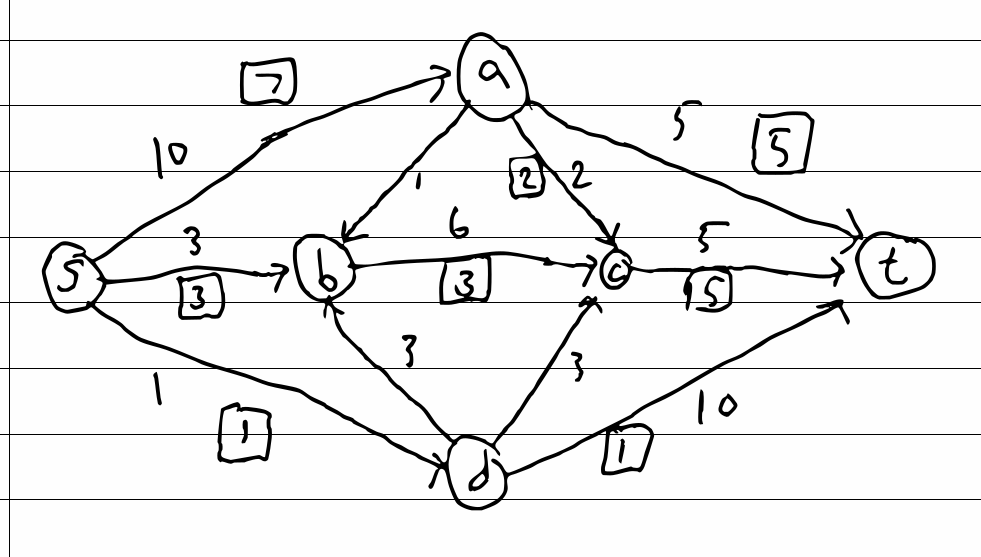
\includegraphics[width=\textwidth]{1a}

    \newpage
    \item The following is the residual graph, $G_f$:
    
    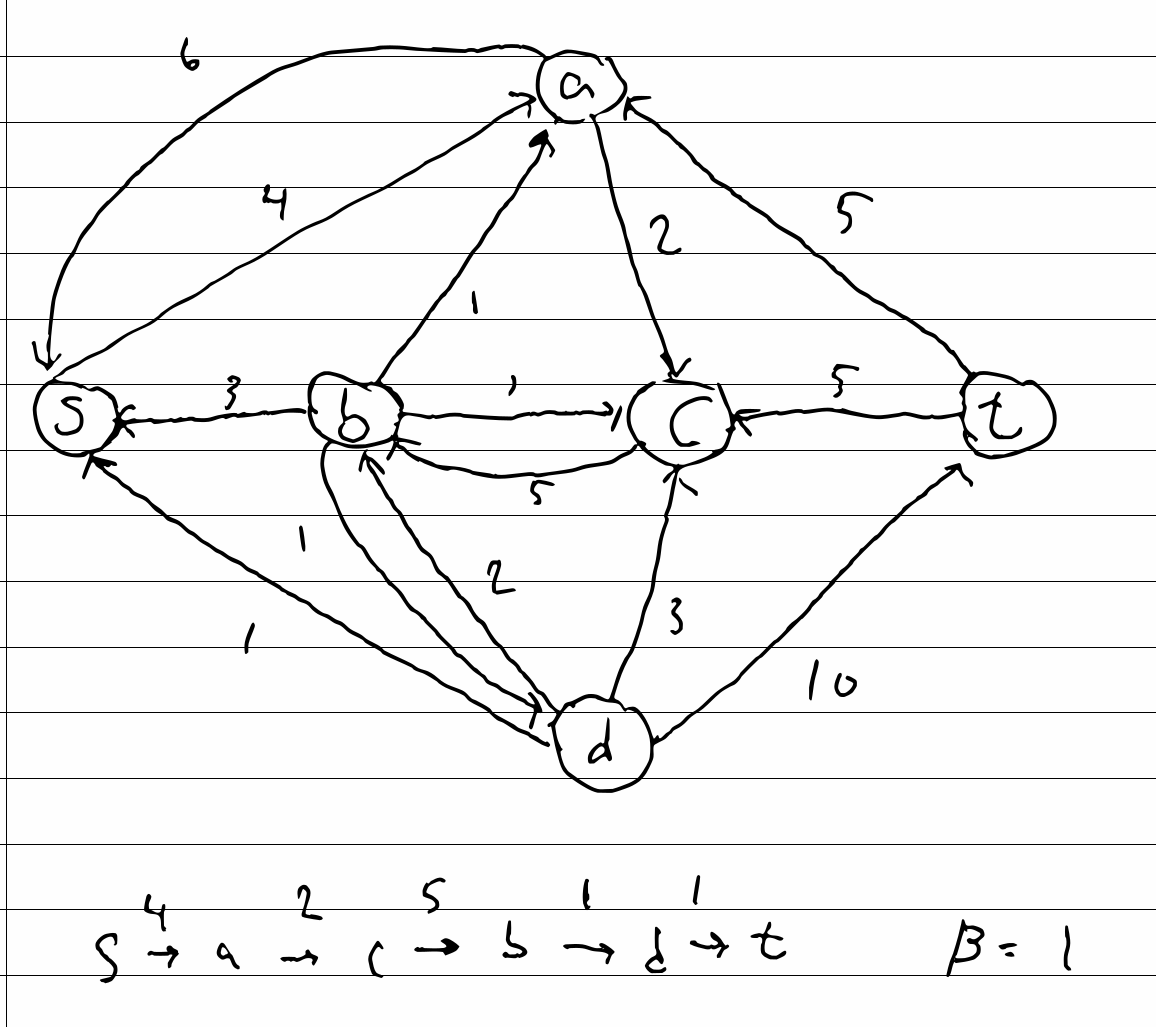
\includegraphics[width=\textwidth]{1b-1}


    We find the augmenting path $P = (s, a, c, b, d, t)$ with a bottleneck of $\beta = 1$ in $G_f$
    We can use this to augment the flow using the \texttt{Augment} procedure to get a flow value of 11:

    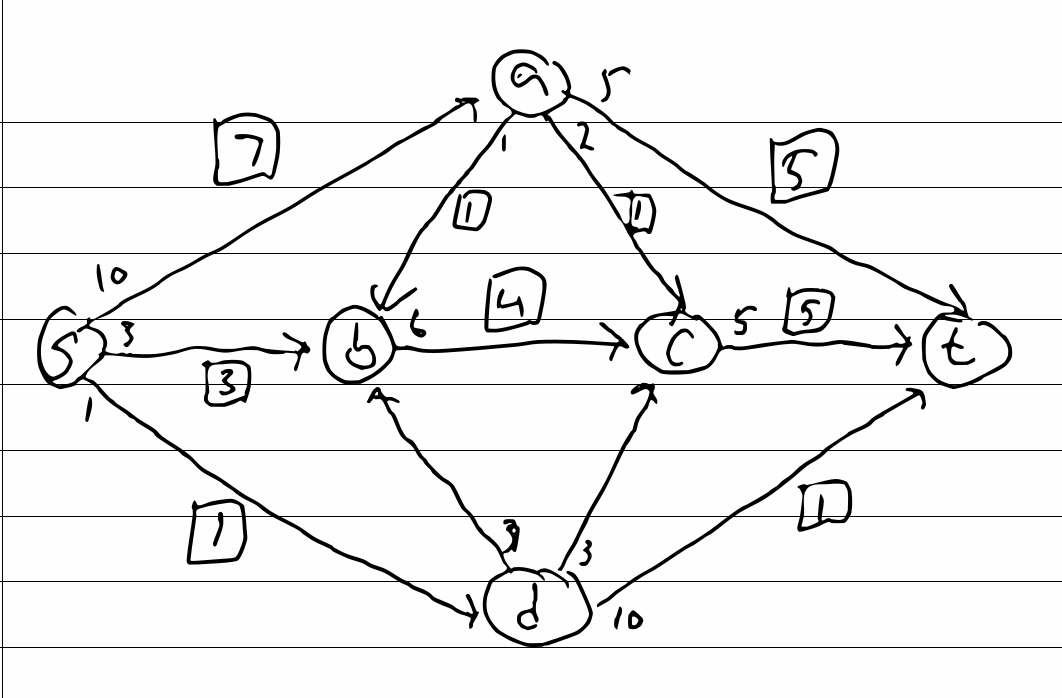
\includegraphics[width=\textwidth]{1b-2}


    This is a maximum flow. We can confirm that by noting that 2 out of the 3 "in" edges are already at capacity $(a, t)$ and $(c, t)$.
    This means in order to increase the flow, we would have to increase the flow at the $(d, t)$ edge. This means $f^{out}(d)$ would have to increase from $f^{out}(d) = 1$.
    But the only "in" edge to $d$ is from the source vertex which has a capacity of 1. That means we cannot increase the flow going through $d$ at all so $11$ is the max flow for the entire graph.

    \item A minimum cut $C(A, B)$ can be done with $A = \{s, a, b, c\}, B = \{d, t\}$ with a capacity of 11.
\end{enumerate}
\newpage
\section{Min Cut}
This is false. Take the following flow below:

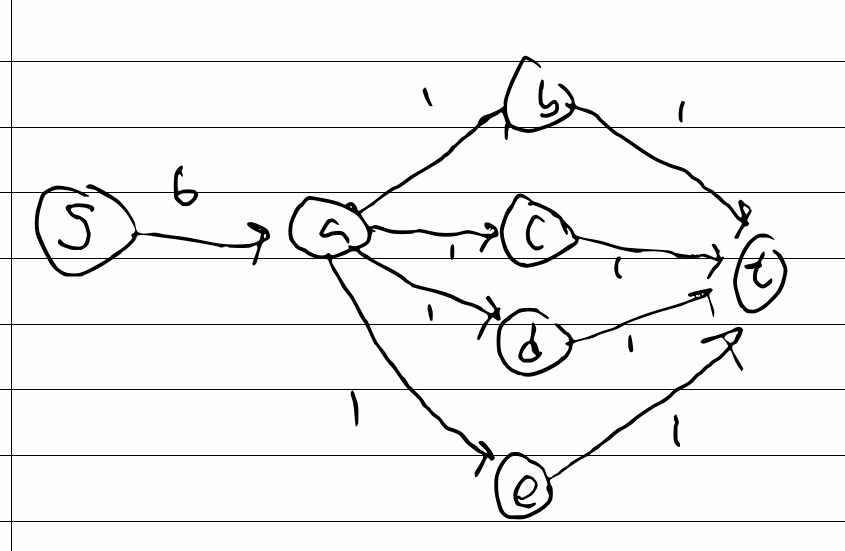
\includegraphics[width=\textwidth]{2_1}


We can construct a minimum cut $(A, B)$ with the following arrangement: $A = \{s, a\}, B = \{b, c, d, e, t\}$.
This cut has a capacity of 4.

Now let's increment all the capacities by 1:

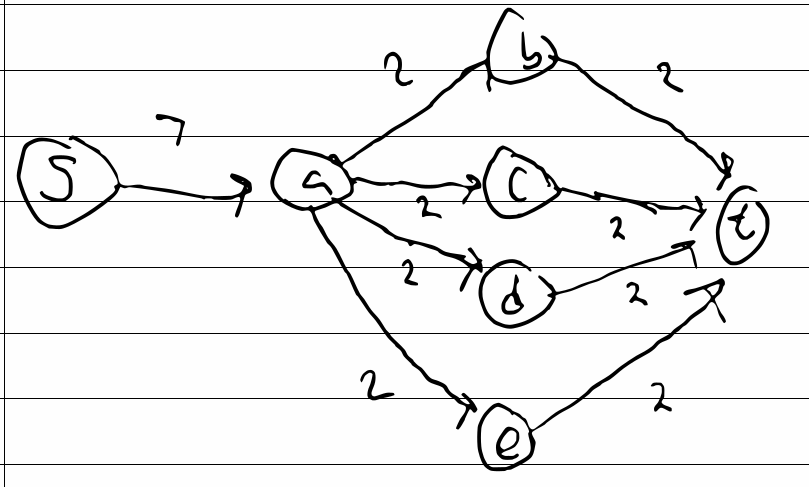
\includegraphics[width=\textwidth]{2_2}

Our old $(A, B)$ cut now has a capacity of 8 but we see that there is a smaller cut available, with a value of 7: 
$A = \{s\}, B = \{a, b, c, d, e, t\}$ so our old cut is no longer the minimium cut.
\newpage

\section{Repairing a Flow}

We first see if the decreased edge was at maximum capacity in flow $f$. If it was not, then we know that decrementing the capacity at this edge will not affect $f$ as $f$ is still a valid flow that follows the capacity principle
and we can return $f$.

Otherwise, we need to run \texttt{Augment} to get the new flow. 
We can do this by first establishing the vertices $u$ and $v$ as the pair of vertices connected by edge $e$.
In order to obey the conservation principle, we use BFS to obtain a path $P1$ from $s$ to $u$ and another BFS to obtain a path $P2$ from $v$ to $t$.
We decrement the flow along $P1$ and $P2$ so that this flow is valid and follows conservation. 
We mark the modified flow with the modified path as $f'$. 
We know $f'$ is a valid flow as $f$ is a valid flow and the only difference between $f$ and $f'$ is that we decremented the capacity of an edge and made sure that that any path using that edge follows conservation.
We can pick any arbitrary path to "fix" as we know any other path going through that edge had followed conservation rules in $f$.

Then, we create the residual graph of this modified flow network, $G'_{f'}$. We can use BFS to try and find an augmenting path in $G'_{f'}$. There are two possibilities here:


\begin{enumerate}
    \item We were lucky when creating $f'$ and this is the new max flow.
    In that case, there is no augmenting path in $G'_{f'}$ and we return $f'$.
    
    \item $f'$ is a valid flow but is not a max flow. In this case, $G'_{f'}$ will contain an augmenting path.
            We call $f'' = \texttt{Augment(f', P)}$ where $P$ is the augmenting path found via BFS.
            Since we only modified the original flow through one path, we know that running \texttt{Augment} once will fix that path and we can return $f''$ which is the new max flow.
\end{enumerate}

We know that we only need to run at most 1 iteration of \texttt{Augment} as we have only modified one path from the original max flow.
Therefore if there is a new max-flow after reducing the edge, we know it will have been at the cause of this new path. This means this new path will contribute to an augmenting path in the residual graph and one iteratin of \texttt{Augment} will find and fix it.  

To get $P1$ and $P2$ we run BFS twice which is $O(|V| + |E|)$ time. Creating the modified $f'$ flow only requires modifying a single path in the original flow so that is also linear time.
Creating the residual graph, running BFS to find an augmenting path, and calling \texttt{Augment} all take linear time as well. Therefore the total runtime of this algorithm is linear: $O(|V| + |E|)$

\newpage
\section{Scheduling Doctors}

We can solve this problem by represnting it as a max flow problem. We can model the problem with a netework graph $G = (V, E)$ as follows:

\begin{align*}
    V &= [k] \cup [n] \cup \{s, t\} \\
    E &= \{\text{ 
        add edges $s \longrightarrow k$  $\forall k\in [k]$ w/ capacity $|L_k|$} \\
      &=  \text{add edges $k \longrightarrow n$  $\forall k\in [k]: (\forall n\in L'_k])$ w/ capacity 1} \\
      &=  \text{add edges $n \longrightarrow t$ $\forall n\in [n]$ w/ capacity $p_n$}\}
\end{align*}

We make a network by creating a sink/source node and a node for every doctor and every day. We connect the source to all the doctor nodes and have an edge capacity of the total number of days that specific doctor is willing to work.
We connect the doctor nodes to the day nodes in a way where only doctors who are willing to work that specific day are connected to that day node with a capacity of 1. 
Then we connect all the day nodes to the sink node with an edge capacity of the required number of doctors needed for that day.

A running flow from a doctor node to a day node represents a doctor working that specific day and the edge leading out of a day node represents the total number of doctors working that specific day.
Therefore to ensure that each day has the required number of doctors, we need to ensure that all edges flowing out of the day nodes are at capacity.

If all outward day nodes are at capacity, we know that we have a max flow from the entire graph by cut intuition. Our cut in this case is $A = V \setminus t $, $B = \{t\}$.
The only input to $t$ is from the outward flow of cut $A$. That means there cannot be a flow that exceeds $A^{out}$.

We can run \texttt{Ford-Fulkerson} on $G$ to obtain the max flow $f$. If the value of the flow $v(f) \neq A^{out}$ (the sum of $(p_1, ...,p_n)$) then we can return that no assignment is possible.

Otherwise, we can create a list of sets representing the days each doctor has to work from $f$.
We do this by examining each doctor node $j$ in $f$. We append every day node $i$ that is connected to doctor $j$ with flow $= 1$ to the set $L'_j$.
Once we are done, we append set $L'_j$ to the main list $L_m$ and we return $L_m$ once every doctor node has been processed.

\subsection{Justification}
This algorithm works as the scheduling doctor problem can be represented as a network graph where a single unit of "flow" is a single "day" that is being worked.
Give an arbitrary network graph $G = (V, E)$ following the construction rules above with $n$ doctors each with their preference list $L_i$ of $k$ days. 
Let $f$ be an arbitrary flow through $G$. 
Let $T \subseteq V$ be the set of doctor nodes and $D \subseteq V$ be the set of day nodes.

From the construction rules listed above, the input capacity for every doctor node is the total number of days they are willing to work.
That means that $f$ will never assign a doctor more days than they are willing to work: $\forall v_i\in T: f^{\text{in}}(v) = f^{\text{out}}(v) \leq |L_i|$
Since the edges from the doctor nodes to the day nodes have capacity 1, a doctor cannot spend multiple of their allocated "flow" days in the same day; they must spread it out across different days.
Since the out edge for all the day nodes have capacity of the requested number of doctors for that day, the flow $f$ will only ever assign a number of doctors less than or equal to the requested amount.
This is how a network graph with a flow is representative of the scheduling doctors problem.

Likewise, given the parameters of a scheduling doctors problem, we can construct a network flow graph given the constraints mentioned in part \textbf{4}.
Solving for the max flow will give us the maximum amount of doctors that can be scheduled in a set of days given the doctors' constraints.

\subsection{Runtime}
Creating the network graph takes $O(n \cdot k)$ time to complete as the worst-case scenario has $n \cdot k + n + k$ edges where every doctor node is connected with every day node.
Running FF takes $O(|E| \cdot C)$ time where $C$ equals the capacity of the max flow as discussed in class.
In this case, the upper-bound of the capacity of the max flow should be $n \cdot k$ in the scenario where everyday requires every doctor.

$O((nk + n + k) \cdot nk) = O((nk)^2)$ 

\newpage
\section{Rearranging a Matrix}

\begin{enumerate}
    \item 
    \begin{align*}
        \begin{vmatrix}
            1 & 0 & 0 \\
            1 & 0 & 0 \\
            0 & 1 & 1
        \end{vmatrix}
    \end{align*}
    
    \item We can solve this problem by reducing it to a problem of checking for a perfect matching in a bipartite graph and solving that as a max flow problem using Ford-Fulkerson. 
    
    We can construct a bipartite graph $G$ of this problem with $V = A \cup B$ where the $n^{\text{th}}$ $a\in A$ represents the $n^{\text{th}}$ row and the $n^{\text{th}}$ $b \in B$ reprsents the $n^{\text{th}}$ column.
    We connect an edge between $(a, b)$ if $M[a, b] = 1$, that is, for each row vertex, we create an edge to a corresponding column vertex if that (row, column) pair is a 1 in the matrix.
        
    As discussed in class, we can reduce this matching problem to a network flow problem and solve for the maximum matching with FF.
    If the size of the maximum matching equals the width of the matrix ($n$), then we know we have a perfect matching and return \True. Otherwise, the matrix is not rearrangeable and we return \False.

    \subsection{Justification}
    First we show that if $G$ has a perfect bipartite matching, its representation of $M$ must be rearrangeable.
    Assume that graph $G$ has a bipartite matching $M_p$. Let's define graph $G' = (V', E')$ as the graph $G$ with only the edges in $M_p$.
    By definition, we know the degree of every $v \in V'$ is 1.
    In our construction of graph $G$, we claimed that the $n^{\text{th}}$ $a\in A$ represents the $n^{\text{th}}$ row of $M$
    and the $n^{\text{th}}$ $b\in B$ represents the $n^{\text{th}}$ column of $M$. Since we can "swap" rows and columns in $M$, we can move the $n^{\text{th}}$ $a\in A$ or $b\in B$ to the $1^{\text{st}}...n^{\text{th}}$ respective location.
    Since we are free to move the positions of $a\in A$ and $b\in B$ as freely as we want, and since $\forall v\in V': d(v) = 1$, we can "line up" each $a\in A$ and $b\in B$ so the $i^{\text{th}}$ $a\in A$ is connected to the $i^{\text{th}}$ $b\in B$.
    Since the presence of an edge means there is a 1 in that $(a, b)$ (column, row), this means our graph $G'$ shows that the $(i, i)$ row column pair has a 1 for i from $[1, n]$. i.e. the matrix has been rearranged to have 1s on the diagonal.

    Now we show that if $M$ is rearrangeable, its graph representation $G = (V, E)$ must have a perfect matching.
    Assume $M$ is rearrangeable. That means that by using some row/column swaps, we can arrive at matrix $M'$ whose diagonals are all 1.
    Let $G' = (V', E')$ be the graph reprsentation of $M'$ following the construction rules listed in \textbf{5.b}.
    Since the diagonals are all 1, we know that in the bipartite subsets, $(a_i, b_i)$ will be an edge in $G'$. 
    This in itself is a perfect bipartite matching. Every $a_i$ is connected to $b_i$. We may add other edges to represent the presence of 1s in non-diagonal locations in $M'$, but we could always erase those edges to reveal the perfect bipartite matching in $G'$. 

    Following the principles of "moving" the $n^{\text{th}}$ $a\in A$ and $n^{\text{th}}$ $b\in B$ as listed above, we know that we can do these "rearrangements" corresponding to the row/column swap operations performed on $M$ to obtain $G$ from $G'$.
    Actually, since this concept of the $n^{\text{th}}$ and $n^{\text{th}}$ $b\in B$ is just an abstraction on graphs we created for this problem (the "order" of vertices in a graph does not matter), we know that $G$ and $G'$ are isophomorphic and practically the same graph (they have the same vertices and same kind of connections between vertices).
    Therefore, we know that $G$ also contains a perfect matching.

    Therefore we have shown that this matrix rearrangement problem can be reduced to a bipartite perfect matching problem.

    \subsection{Runtime}
    To create $G$, we need to investigate every element in every row of $M$ which takes $O(n^2)$ across the entire matrix.
    Ford-Fulkerson takes $O(|E| \cdot C)$ as discussed in class. The maximum amount of edges in $G$ is $n^2$ where $\forall a\in A, \forall b\in B: (a, b) \in E$ (the entire matrix is full of 1s).
    The maximum max-flow in a bipartite construction like this is in a perfect matching where max-flow is $n$.
    
    That means running FF will take $O(n^3)$ time so the runtime of the entire algorithm is $O(n^3)$

\end{enumerate}
\end{document}
